\documentclass[twoside]{book}

% Packages required by doxygen
\usepackage{fixltx2e}
\usepackage{calc}
\usepackage{doxygen}
\usepackage[export]{adjustbox} % also loads graphicx
\usepackage{graphicx}
\usepackage[utf8]{inputenc}
\usepackage{makeidx}
\usepackage{multicol}
\usepackage{multirow}
\PassOptionsToPackage{warn}{textcomp}
\usepackage{textcomp}
\usepackage[nointegrals]{wasysym}
\usepackage[table]{xcolor}

% Font selection
\usepackage[T1]{fontenc}
\usepackage[scaled=.90]{helvet}
\usepackage{courier}
\usepackage{amssymb}
\usepackage{sectsty}
\renewcommand{\familydefault}{\sfdefault}
\allsectionsfont{%
  \fontseries{bc}\selectfont%
  \color{darkgray}%
}
\renewcommand{\DoxyLabelFont}{%
  \fontseries{bc}\selectfont%
  \color{darkgray}%
}
\newcommand{\+}{\discretionary{\mbox{\scriptsize$\hookleftarrow$}}{}{}}

% Page & text layout
\usepackage{geometry}
\geometry{%
  a4paper,%
  top=2.5cm,%
  bottom=2.5cm,%
  left=2.5cm,%
  right=2.5cm%
}
\tolerance=750
\hfuzz=15pt
\hbadness=750
\setlength{\emergencystretch}{15pt}
\setlength{\parindent}{0cm}
\setlength{\parskip}{3ex plus 2ex minus 2ex}
\makeatletter
\renewcommand{\paragraph}{%
  \@startsection{paragraph}{4}{0ex}{-1.0ex}{1.0ex}{%
    \normalfont\normalsize\bfseries\SS@parafont%
  }%
}
\renewcommand{\subparagraph}{%
  \@startsection{subparagraph}{5}{0ex}{-1.0ex}{1.0ex}{%
    \normalfont\normalsize\bfseries\SS@subparafont%
  }%
}
\makeatother

% Headers & footers
\usepackage{fancyhdr}
\pagestyle{fancyplain}
\fancyhead[LE]{\fancyplain{}{\bfseries\thepage}}
\fancyhead[CE]{\fancyplain{}{}}
\fancyhead[RE]{\fancyplain{}{\bfseries\leftmark}}
\fancyhead[LO]{\fancyplain{}{\bfseries\rightmark}}
\fancyhead[CO]{\fancyplain{}{}}
\fancyhead[RO]{\fancyplain{}{\bfseries\thepage}}
\fancyfoot[LE]{\fancyplain{}{}}
\fancyfoot[CE]{\fancyplain{}{}}
\fancyfoot[RE]{\fancyplain{}{\bfseries\scriptsize Generated by Doxygen }}
\fancyfoot[LO]{\fancyplain{}{\bfseries\scriptsize Generated by Doxygen }}
\fancyfoot[CO]{\fancyplain{}{}}
\fancyfoot[RO]{\fancyplain{}{}}
\renewcommand{\footrulewidth}{0.4pt}
\renewcommand{\chaptermark}[1]{%
  \markboth{#1}{}%
}
\renewcommand{\sectionmark}[1]{%
  \markright{\thesection\ #1}%
}

% Indices & bibliography
\usepackage{natbib}
\usepackage[titles]{tocloft}
\setcounter{tocdepth}{3}
\setcounter{secnumdepth}{5}
\makeindex

% Hyperlinks (required, but should be loaded last)
\usepackage{ifpdf}
\ifpdf
  \usepackage[pdftex,pagebackref=true]{hyperref}
\else
  \usepackage[ps2pdf,pagebackref=true]{hyperref}
\fi
\hypersetup{%
  colorlinks=true,%
  linkcolor=blue,%
  citecolor=blue,%
  unicode%
}

% Custom commands
\newcommand{\clearemptydoublepage}{%
  \newpage{\pagestyle{empty}\cleardoublepage}%
}

\usepackage{caption}
\captionsetup{labelsep=space,justification=centering,font={bf},singlelinecheck=off,skip=4pt,position=top}

%===== C O N T E N T S =====

\begin{document}

% Titlepage & ToC
\hypersetup{pageanchor=false,
             bookmarksnumbered=true,
             pdfencoding=unicode
            }
\pagenumbering{alph}
\begin{titlepage}
\vspace*{7cm}
\begin{center}%
{\Large My Project }\\
\vspace*{1cm}
{\large Generated by Doxygen 1.8.13}\\
\end{center}
\end{titlepage}
\clearemptydoublepage
\pagenumbering{roman}
\tableofcontents
\clearemptydoublepage
\pagenumbering{arabic}
\hypersetup{pageanchor=true}

%--- Begin generated contents ---
\chapter{Hierarchical Index}
\section{Class Hierarchy}
This inheritance list is sorted roughly, but not completely, alphabetically\+:\begin{DoxyCompactList}
\item Q\+File\+Info\begin{DoxyCompactList}
\item \contentsline{section}{Playlist\+Item}{\pageref{classPlaylistItem}}{}
\end{DoxyCompactList}
\item Q\+List\+Widget\begin{DoxyCompactList}
\item \contentsline{section}{Playlist}{\pageref{classPlaylist}}{}
\end{DoxyCompactList}
\item Q\+List\+Widget\+Item\begin{DoxyCompactList}
\item \contentsline{section}{Playlist\+Item}{\pageref{classPlaylistItem}}{}
\end{DoxyCompactList}
\item Q\+Main\+Window\begin{DoxyCompactList}
\item \contentsline{section}{Main\+Window}{\pageref{classMainWindow}}{}
\end{DoxyCompactList}
\item Q\+Push\+Button\begin{DoxyCompactList}
\item \contentsline{section}{Multi\+Icon\+Button}{\pageref{classMultiIconButton}}{}
\end{DoxyCompactList}
\item Q\+Slider\begin{DoxyCompactList}
\item \contentsline{section}{Clickable\+Slider}{\pageref{classClickableSlider}}{}
\end{DoxyCompactList}
\item Q\+Widget\begin{DoxyCompactList}
\item \contentsline{section}{Status\+Bar}{\pageref{classStatusBar}}{}
\end{DoxyCompactList}
\end{DoxyCompactList}

\chapter{Class Index}
\section{Class List}
Here are the classes, structs, unions and interfaces with brief descriptions\+:\begin{DoxyCompactList}
\item\contentsline{section}{\hyperlink{classClickableSlider}{Clickable\+Slider} \\*A simple reimplementation of the Q\+Slider class, where clicking on the slider will change the returned value }{\pageref{classClickableSlider}}{}
\item\contentsline{section}{\hyperlink{classMainWindow}{Main\+Window} }{\pageref{classMainWindow}}{}
\item\contentsline{section}{\hyperlink{classMultiIconButton}{Multi\+Icon\+Button} }{\pageref{classMultiIconButton}}{}
\item\contentsline{section}{\hyperlink{classPlaylist}{Playlist} }{\pageref{classPlaylist}}{}
\item\contentsline{section}{\hyperlink{classPlaylistItem}{Playlist\+Item} }{\pageref{classPlaylistItem}}{}
\item\contentsline{section}{\hyperlink{classStatusBar}{Status\+Bar} \\*Concatenation of 2 Q\+Labels and a \hyperlink{classClickableSlider}{Clickable\+Slider}, in order to display the progression of the played media, and the signals and slots to handle it }{\pageref{classStatusBar}}{}
\end{DoxyCompactList}

\chapter{Class Documentation}
\hypertarget{classClickableSlider}{}\section{Clickable\+Slider Class Reference}
\label{classClickableSlider}\index{Clickable\+Slider@{Clickable\+Slider}}


A simple reimplementation of the Q\+Slider class, where clicking on the slider will change the returned value.  




{\ttfamily \#include $<$statusbar.\+h$>$}



Inheritance diagram for Clickable\+Slider\+:\nopagebreak
\begin{figure}[H]
\begin{center}
\leavevmode
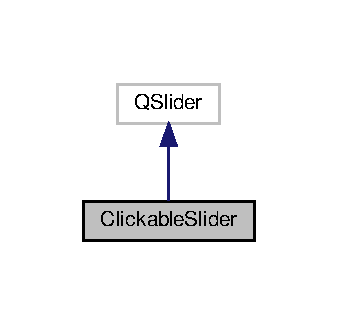
\includegraphics[width=162pt]{classClickableSlider__inherit__graph}
\end{center}
\end{figure}


Collaboration diagram for Clickable\+Slider\+:\nopagebreak
\begin{figure}[H]
\begin{center}
\leavevmode
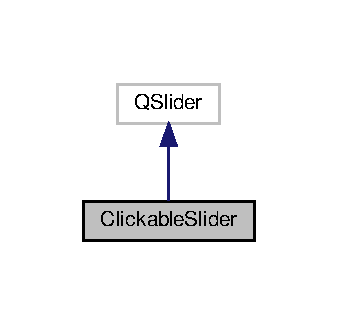
\includegraphics[width=162pt]{classClickableSlider__coll__graph}
\end{center}
\end{figure}
\subsection*{Public Member Functions}
\begin{DoxyCompactItemize}
\item 
\hyperlink{classClickableSlider_a049ecbf035b3dc9c5521832fb9ae941b}{Clickable\+Slider} (Q\+Widget $\ast$parent=nullptr)
\begin{DoxyCompactList}\small\item\em just a empty constructor, just here to call the Q\+Slider constructor \end{DoxyCompactList}\item 
void \hyperlink{classClickableSlider_aa71c72cea3732cb9e8753bd64305d913}{mouse\+Press\+Event} (Q\+Mouse\+Event $\ast$event)
\begin{DoxyCompactList}\small\item\em The method this class was created for, changing the value of the slider in function of the click of the mouse. Only the left click has an effect. \end{DoxyCompactList}\end{DoxyCompactItemize}


\subsection{Detailed Description}
A simple reimplementation of the Q\+Slider class, where clicking on the slider will change the returned value. 

\subsection{Constructor \& Destructor Documentation}
\mbox{\Hypertarget{classClickableSlider_a049ecbf035b3dc9c5521832fb9ae941b}\label{classClickableSlider_a049ecbf035b3dc9c5521832fb9ae941b}} 
\index{Clickable\+Slider@{Clickable\+Slider}!Clickable\+Slider@{Clickable\+Slider}}
\index{Clickable\+Slider@{Clickable\+Slider}!Clickable\+Slider@{Clickable\+Slider}}
\subsubsection{\texorpdfstring{Clickable\+Slider()}{ClickableSlider()}}
{\footnotesize\ttfamily Clickable\+Slider\+::\+Clickable\+Slider (\begin{DoxyParamCaption}\item[{Q\+Widget $\ast$}]{parent = {\ttfamily nullptr} }\end{DoxyParamCaption})}



just a empty constructor, just here to call the Q\+Slider constructor 


\begin{DoxyParams}{Parameters}
{\em parent} & a pointer to the Q\+Widget who include this slider, null by default \\
\hline
\end{DoxyParams}


\subsection{Member Function Documentation}
\mbox{\Hypertarget{classClickableSlider_aa71c72cea3732cb9e8753bd64305d913}\label{classClickableSlider_aa71c72cea3732cb9e8753bd64305d913}} 
\index{Clickable\+Slider@{Clickable\+Slider}!mouse\+Press\+Event@{mouse\+Press\+Event}}
\index{mouse\+Press\+Event@{mouse\+Press\+Event}!Clickable\+Slider@{Clickable\+Slider}}
\subsubsection{\texorpdfstring{mouse\+Press\+Event()}{mousePressEvent()}}
{\footnotesize\ttfamily void Clickable\+Slider\+::mouse\+Press\+Event (\begin{DoxyParamCaption}\item[{Q\+Mouse\+Event $\ast$}]{event }\end{DoxyParamCaption})}



The method this class was created for, changing the value of the slider in function of the click of the mouse. Only the left click has an effect. 


\begin{DoxyParams}{Parameters}
{\em event} & the mouse event \\
\hline
\end{DoxyParams}


The documentation for this class was generated from the following files\+:\begin{DoxyCompactItemize}
\item 
statusbar.\+h\item 
statusbar.\+cpp\end{DoxyCompactItemize}

\hypertarget{classMainWindow}{}\section{Main\+Window Class Reference}
\label{classMainWindow}\index{Main\+Window@{Main\+Window}}


Inheritance diagram for Main\+Window\+:\nopagebreak
\begin{figure}[H]
\begin{center}
\leavevmode
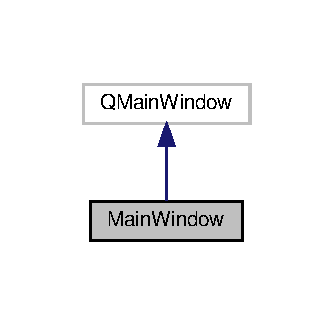
\includegraphics[width=160pt]{classMainWindow__inherit__graph}
\end{center}
\end{figure}


Collaboration diagram for Main\+Window\+:\nopagebreak
\begin{figure}[H]
\begin{center}
\leavevmode
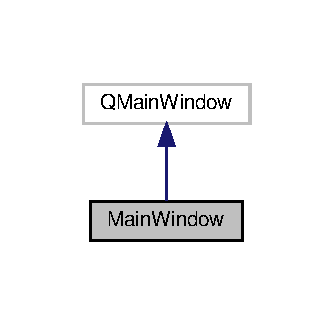
\includegraphics[width=160pt]{classMainWindow__coll__graph}
\end{center}
\end{figure}
\subsection*{Signals}
\begin{DoxyCompactItemize}
\item 
\mbox{\Hypertarget{classMainWindow_a8981ec6b1564821c10b2db484556c335}\label{classMainWindow_a8981ec6b1564821c10b2db484556c335}} 
void {\bfseries play} (void)
\item 
\mbox{\Hypertarget{classMainWindow_ad36b52312116711a1c0e88917b07cea3}\label{classMainWindow_ad36b52312116711a1c0e88917b07cea3}} 
void {\bfseries pause} (void)
\item 
\mbox{\Hypertarget{classMainWindow_a003efa6afe9f5cb7c0bc73dada912e80}\label{classMainWindow_a003efa6afe9f5cb7c0bc73dada912e80}} 
void {\bfseries stop} (void)
\end{DoxyCompactItemize}
\subsection*{Public Member Functions}
\begin{DoxyCompactItemize}
\item 
\mbox{\Hypertarget{classMainWindow_a996c5a2b6f77944776856f08ec30858d}\label{classMainWindow_a996c5a2b6f77944776856f08ec30858d}} 
{\bfseries Main\+Window} (Q\+Widget $\ast$parent=nullptr)
\end{DoxyCompactItemize}


The documentation for this class was generated from the following files\+:\begin{DoxyCompactItemize}
\item 
mainwindow.\+h\item 
mainwindow.\+cpp\end{DoxyCompactItemize}

\hypertarget{classMultiIconButton}{}\section{Multi\+Icon\+Button Class Reference}
\label{classMultiIconButton}\index{Multi\+Icon\+Button@{Multi\+Icon\+Button}}


Inheritance diagram for Multi\+Icon\+Button\+:\nopagebreak
\begin{figure}[H]
\begin{center}
\leavevmode
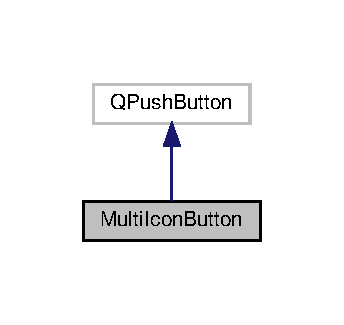
\includegraphics[width=165pt]{classMultiIconButton__inherit__graph}
\end{center}
\end{figure}


Collaboration diagram for Multi\+Icon\+Button\+:\nopagebreak
\begin{figure}[H]
\begin{center}
\leavevmode
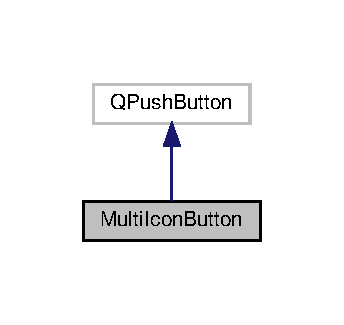
\includegraphics[width=165pt]{classMultiIconButton__coll__graph}
\end{center}
\end{figure}
\subsection*{Public Member Functions}
\begin{DoxyCompactItemize}
\item 
\mbox{\Hypertarget{classMultiIconButton_af5b082899f26d24b401106b5c7ea7082}\label{classMultiIconButton_af5b082899f26d24b401106b5c7ea7082}} 
{\bfseries Multi\+Icon\+Button} (Q\+Widget $\ast$parent=nullptr)
\item 
\mbox{\Hypertarget{classMultiIconButton_a52dea076e62b15d50650ca40c7d61a87}\label{classMultiIconButton_a52dea076e62b15d50650ca40c7d61a87}} 
{\bfseries Multi\+Icon\+Button} (const Q\+Icon \&icon, const Q\+String \&text, Q\+Widget $\ast$parent=nullptr)
\item 
\mbox{\Hypertarget{classMultiIconButton_abc95c922c89a0835470342cad3c0ea7f}\label{classMultiIconButton_abc95c922c89a0835470342cad3c0ea7f}} 
void {\bfseries add\+Icon} (const Q\+Icon \&icon)
\item 
\mbox{\Hypertarget{classMultiIconButton_ac2f861763803393327d207ff07892f96}\label{classMultiIconButton_ac2f861763803393327d207ff07892f96}} 
void {\bfseries switch\+Icon} (void)
\item 
\mbox{\Hypertarget{classMultiIconButton_aeefcca86f41e97b5042f335e75b414d0}\label{classMultiIconButton_aeefcca86f41e97b5042f335e75b414d0}} 
void {\bfseries set\+Icon} (const Q\+Icon \&icon)
\end{DoxyCompactItemize}


The documentation for this class was generated from the following files\+:\begin{DoxyCompactItemize}
\item 
multiiconbutton.\+h\item 
multiiconbutton.\+cpp\end{DoxyCompactItemize}

\hypertarget{classPlaylist}{}\section{Playlist Class Reference}
\label{classPlaylist}\index{Playlist@{Playlist}}


Inheritance diagram for Playlist\+:\nopagebreak
\begin{figure}[H]
\begin{center}
\leavevmode
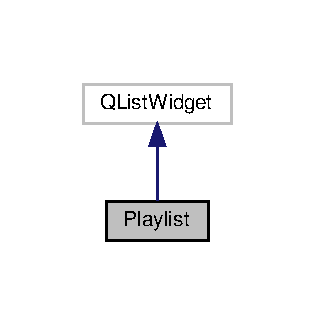
\includegraphics[width=151pt]{classPlaylist__inherit__graph}
\end{center}
\end{figure}


Collaboration diagram for Playlist\+:\nopagebreak
\begin{figure}[H]
\begin{center}
\leavevmode
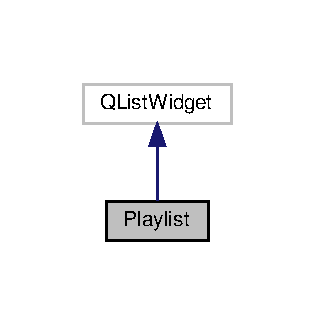
\includegraphics[width=151pt]{classPlaylist__coll__graph}
\end{center}
\end{figure}
\subsection*{Signals}
\begin{DoxyCompactItemize}
\item 
\mbox{\Hypertarget{classPlaylist_ad3fb0ec925f1ba71c7ca8d3152645c4a}\label{classPlaylist_ad3fb0ec925f1ba71c7ca8d3152645c4a}} 
void {\bfseries item\+Double\+Clicked} (\hyperlink{classPlaylistItem}{Playlist\+Item} $\ast$item)
\item 
\mbox{\Hypertarget{classPlaylist_a0a4a4754313dd19270cd43c9a3671bdc}\label{classPlaylist_a0a4a4754313dd19270cd43c9a3671bdc}} 
void {\bfseries item\+Clicked} (\hyperlink{classPlaylistItem}{Playlist\+Item} $\ast$item)
\end{DoxyCompactItemize}
\subsection*{Public Member Functions}
\begin{DoxyCompactItemize}
\item 
\mbox{\Hypertarget{classPlaylist_a1a38dac71a234491bc933bd5089c54b0}\label{classPlaylist_a1a38dac71a234491bc933bd5089c54b0}} 
{\bfseries Playlist} (Q\+Widget $\ast$parent=nullptr)
\item 
\mbox{\Hypertarget{classPlaylist_a1277d4881eeaad2562ff883fa7b90833}\label{classPlaylist_a1277d4881eeaad2562ff883fa7b90833}} 
void {\bfseries add\+Item} (\hyperlink{classPlaylistItem}{Playlist\+Item} $\ast$item)
\item 
\mbox{\Hypertarget{classPlaylist_a1a8512bea74f92bac13d8827dec1a6ac}\label{classPlaylist_a1a8512bea74f92bac13d8827dec1a6ac}} 
void {\bfseries add\+Item} (Q\+String path)
\item 
\mbox{\Hypertarget{classPlaylist_a0b6ccc713cf25550bc5fac2cef666e5d}\label{classPlaylist_a0b6ccc713cf25550bc5fac2cef666e5d}} 
void {\bfseries add\+Items} (Q\+String\+List paths)
\item 
\mbox{\Hypertarget{classPlaylist_a31b754a62bccbd79b6a5320d02ca50f3}\label{classPlaylist_a31b754a62bccbd79b6a5320d02ca50f3}} 
\hyperlink{classPlaylistItem}{Playlist\+Item} $\ast$ {\bfseries item} (int index)
\item 
\mbox{\Hypertarget{classPlaylist_a9fb676932435eb9c599d82e1e0e2e919}\label{classPlaylist_a9fb676932435eb9c599d82e1e0e2e919}} 
\hyperlink{classPlaylistItem}{Playlist\+Item} $\ast$ {\bfseries current\+Item} (void)
\item 
\mbox{\Hypertarget{classPlaylist_af38010d3b29b01bfd4e06a25a9f91484}\label{classPlaylist_af38010d3b29b01bfd4e06a25a9f91484}} 
\hyperlink{classPlaylistItem}{Playlist\+Item} $\ast$ {\bfseries take\+Item} (int index)
\item 
\mbox{\Hypertarget{classPlaylist_a8d9b899e88674cde1d6158cef5244c96}\label{classPlaylist_a8d9b899e88674cde1d6158cef5244c96}} 
void {\bfseries insert\+Item} (int index, \hyperlink{classPlaylistItem}{Playlist\+Item} $\ast$item)
\end{DoxyCompactItemize}


The documentation for this class was generated from the following files\+:\begin{DoxyCompactItemize}
\item 
playlist.\+h\item 
playlist.\+cpp\end{DoxyCompactItemize}

\hypertarget{classPlaylistItem}{}\section{Playlist\+Item Class Reference}
\label{classPlaylistItem}\index{Playlist\+Item@{Playlist\+Item}}


Inheritance diagram for Playlist\+Item\+:\nopagebreak
\begin{figure}[H]
\begin{center}
\leavevmode
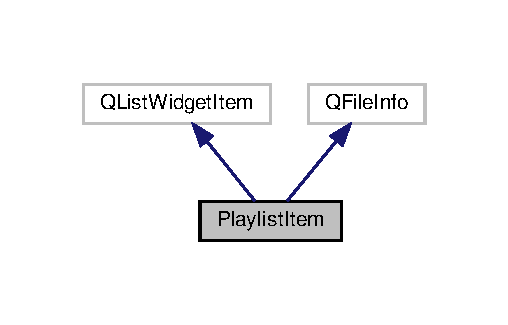
\includegraphics[width=244pt]{classPlaylistItem__inherit__graph}
\end{center}
\end{figure}


Collaboration diagram for Playlist\+Item\+:\nopagebreak
\begin{figure}[H]
\begin{center}
\leavevmode
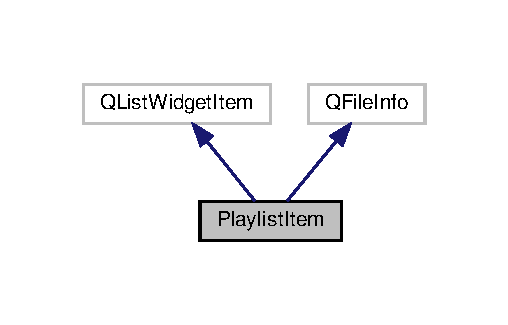
\includegraphics[width=244pt]{classPlaylistItem__coll__graph}
\end{center}
\end{figure}
\subsection*{Public Member Functions}
\begin{DoxyCompactItemize}
\item 
\mbox{\Hypertarget{classPlaylistItem_ab7983fead6752aa8795868c8f4f3ce32}\label{classPlaylistItem_ab7983fead6752aa8795868c8f4f3ce32}} 
{\bfseries Playlist\+Item} (Q\+String path)
\end{DoxyCompactItemize}


The documentation for this class was generated from the following files\+:\begin{DoxyCompactItemize}
\item 
playlist.\+h\item 
playlist.\+cpp\end{DoxyCompactItemize}

\hypertarget{classStatusBar}{}\section{Status\+Bar Class Reference}
\label{classStatusBar}\index{Status\+Bar@{Status\+Bar}}


a concatenation of 2 Q\+Labels and a \hyperlink{classClickableSlider}{Clickable\+Slider}, in order to display the progression of the played media, and the signals and slots to handle it  




{\ttfamily \#include $<$statusbar.\+h$>$}



Inheritance diagram for Status\+Bar\+:\nopagebreak
\begin{figure}[H]
\begin{center}
\leavevmode
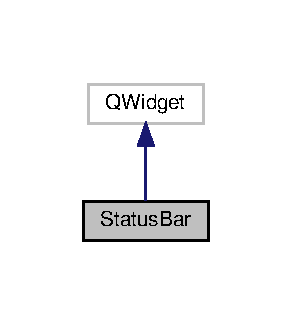
\includegraphics[width=140pt]{classStatusBar__inherit__graph}
\end{center}
\end{figure}


Collaboration diagram for Status\+Bar\+:\nopagebreak
\begin{figure}[H]
\begin{center}
\leavevmode
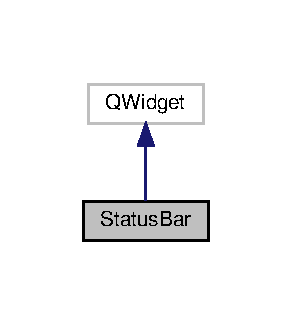
\includegraphics[width=140pt]{classStatusBar__coll__graph}
\end{center}
\end{figure}
\subsection*{Public Slots}
\begin{DoxyCompactItemize}
\item 
void \hyperlink{classStatusBar_af2f6ab9ea87a5337e9dad2bb39c0bb15}{duration\+Changed} (qint64 duration)
\begin{DoxyCompactList}\small\item\em A slot to handle the signal launch by the player, when the currently read media duration has changed, a duration null, the first one send by player for every media, is ignored. \end{DoxyCompactList}\item 
\mbox{\Hypertarget{classStatusBar_a9f002b8c9a2d5c48260a0ebbad12f9df}\label{classStatusBar_a9f002b8c9a2d5c48260a0ebbad12f9df}} 
void \hyperlink{classStatusBar_a9f002b8c9a2d5c48260a0ebbad12f9df}{elapsed\+Second} (void)
\begin{DoxyCompactList}\small\item\em A slot to handle the internal timer signal every second, increasing elapsed time, decreasing remaining time, and changing the Qlabels and the \hyperlink{classClickableSlider}{Clickable\+Slider} displayed times. \end{DoxyCompactList}\item 
\mbox{\Hypertarget{classStatusBar_a3c4e217b69264cb6b07f587af9767209}\label{classStatusBar_a3c4e217b69264cb6b07f587af9767209}} 
void \hyperlink{classStatusBar_a3c4e217b69264cb6b07f587af9767209}{start} (void)
\begin{DoxyCompactList}\small\item\em A slot to handle the play signal of the \hyperlink{classMainWindow}{Main\+Window}. \end{DoxyCompactList}\item 
\mbox{\Hypertarget{classStatusBar_ae5c8930a2b9ec0b88c48dec8f46a55d5}\label{classStatusBar_ae5c8930a2b9ec0b88c48dec8f46a55d5}} 
void \hyperlink{classStatusBar_ae5c8930a2b9ec0b88c48dec8f46a55d5}{pause} (void)
\begin{DoxyCompactList}\small\item\em A slot to handle the pause signal of the \hyperlink{classMainWindow}{Main\+Window}. \end{DoxyCompactList}\item 
\mbox{\Hypertarget{classStatusBar_af52f3efb90d4c83a5602dbbf210e8d79}\label{classStatusBar_af52f3efb90d4c83a5602dbbf210e8d79}} 
void \hyperlink{classStatusBar_af52f3efb90d4c83a5602dbbf210e8d79}{reset} (void)
\begin{DoxyCompactList}\small\item\em A slot to handle the stop signal of the \hyperlink{classMainWindow}{Main\+Window}, reseting the displayed times. \end{DoxyCompactList}\item 
\mbox{\Hypertarget{classStatusBar_aa36e38a90475a85dc8d84b31efc4e834}\label{classStatusBar_aa36e38a90475a85dc8d84b31efc4e834}} 
void \hyperlink{classStatusBar_aa36e38a90475a85dc8d84b31efc4e834}{value\+Changed} (void)
\begin{DoxyCompactList}\small\item\em A slot to handle the value\+Changed signal of the \hyperlink{classClickableSlider}{Clickable\+Slider}. \end{DoxyCompactList}\item 
void \hyperlink{classStatusBar_a58be568ef32791d26f2d45063189c4af}{state\+Changed} (Q\+Media\+Player\+::\+State state)
\begin{DoxyCompactList}\small\item\em A slot to handle the signal send by the player, when the read media is changed. \end{DoxyCompactList}\item 
\mbox{\Hypertarget{classStatusBar_a7beb68db1b57bc79cb2502239ebc7585}\label{classStatusBar_a7beb68db1b57bc79cb2502239ebc7585}} 
void \hyperlink{classStatusBar_a7beb68db1b57bc79cb2502239ebc7585}{clear} (void)
\begin{DoxyCompactList}\small\item\em A slot to handle the absence of any media read by the player. \end{DoxyCompactList}\end{DoxyCompactItemize}
\subsection*{Signals}
\begin{DoxyCompactItemize}
\item 
void \hyperlink{classStatusBar_adf37ac3b2bf684e9d9d53c8ea345b0b9}{set\+Position} (qint64 new\+Position)
\begin{DoxyCompactList}\small\item\em A signal send to the player to change the second played in the currently read media. \end{DoxyCompactList}\end{DoxyCompactItemize}
\subsection*{Public Member Functions}
\begin{DoxyCompactItemize}
\item 
\hyperlink{classStatusBar_a51d704471d7c6b35567bf325bea87cfa}{Status\+Bar} (Q\+Widget $\ast$parent=nullptr)
\begin{DoxyCompactList}\small\item\em The constructor, creating the internal timer and setting every internal variables to 0. \end{DoxyCompactList}\item 
void \hyperlink{classStatusBar_aec9c453a499cd3737f7dd24903aae133}{set\+Slider} (\hyperlink{classClickableSlider}{Clickable\+Slider} $\ast$slider)
\begin{DoxyCompactList}\small\item\em The setter for the \hyperlink{classClickableSlider}{Clickable\+Slider}, it also connect the slider\textquotesingle{}s signal for a changed value to the class slot to handle it. \end{DoxyCompactList}\item 
void \hyperlink{classStatusBar_a285ff0279e3f9d5b677d83ce236f6d25}{set\+Elapsed\+Time\+Label} (Q\+Label $\ast$label)
\begin{DoxyCompactList}\small\item\em The setter for the Q\+Label displaying the elapsed time of the currently read media, this also set the displayed time to 00\+:00. \end{DoxyCompactList}\item 
void \hyperlink{classStatusBar_af8e70f7ce434b29b04a5aaced2dd05ae}{set\+Remaining\+Time\+Label} (Q\+Label $\ast$label)
\begin{DoxyCompactList}\small\item\em The setter for the Q\+L\+Abel displaying the remaining time of the currently read media, this also set the displayed time to 00\+:00. \end{DoxyCompactList}\end{DoxyCompactItemize}


\subsection{Detailed Description}
a concatenation of 2 Q\+Labels and a \hyperlink{classClickableSlider}{Clickable\+Slider}, in order to display the progression of the played media, and the signals and slots to handle it 

\subsection{Constructor \& Destructor Documentation}
\mbox{\Hypertarget{classStatusBar_a51d704471d7c6b35567bf325bea87cfa}\label{classStatusBar_a51d704471d7c6b35567bf325bea87cfa}} 
\index{Status\+Bar@{Status\+Bar}!Status\+Bar@{Status\+Bar}}
\index{Status\+Bar@{Status\+Bar}!Status\+Bar@{Status\+Bar}}
\subsubsection{\texorpdfstring{Status\+Bar()}{StatusBar()}}
{\footnotesize\ttfamily Status\+Bar\+::\+Status\+Bar (\begin{DoxyParamCaption}\item[{Q\+Widget $\ast$}]{parent = {\ttfamily nullptr} }\end{DoxyParamCaption})}



The constructor, creating the internal timer and setting every internal variables to 0. 


\begin{DoxyParams}{Parameters}
{\em parent} & the Q\+Widget where this object is displayed, null by default \\
\hline
\end{DoxyParams}


\subsection{Member Function Documentation}
\mbox{\Hypertarget{classStatusBar_af2f6ab9ea87a5337e9dad2bb39c0bb15}\label{classStatusBar_af2f6ab9ea87a5337e9dad2bb39c0bb15}} 
\index{Status\+Bar@{Status\+Bar}!duration\+Changed@{duration\+Changed}}
\index{duration\+Changed@{duration\+Changed}!Status\+Bar@{Status\+Bar}}
\subsubsection{\texorpdfstring{duration\+Changed}{durationChanged}}
{\footnotesize\ttfamily void Status\+Bar\+::duration\+Changed (\begin{DoxyParamCaption}\item[{qint64}]{duration }\end{DoxyParamCaption})\hspace{0.3cm}{\ttfamily [slot]}}



A slot to handle the signal launch by the player, when the currently read media duration has changed, a duration null, the first one send by player for every media, is ignored. 


\begin{DoxyParams}{Parameters}
{\em duration} & the media duration, in milliseconds \\
\hline
\end{DoxyParams}
\mbox{\Hypertarget{classStatusBar_a285ff0279e3f9d5b677d83ce236f6d25}\label{classStatusBar_a285ff0279e3f9d5b677d83ce236f6d25}} 
\index{Status\+Bar@{Status\+Bar}!set\+Elapsed\+Time\+Label@{set\+Elapsed\+Time\+Label}}
\index{set\+Elapsed\+Time\+Label@{set\+Elapsed\+Time\+Label}!Status\+Bar@{Status\+Bar}}
\subsubsection{\texorpdfstring{set\+Elapsed\+Time\+Label()}{setElapsedTimeLabel()}}
{\footnotesize\ttfamily void Status\+Bar\+::set\+Elapsed\+Time\+Label (\begin{DoxyParamCaption}\item[{Q\+Label $\ast$}]{label }\end{DoxyParamCaption})}



The setter for the Q\+Label displaying the elapsed time of the currently read media, this also set the displayed time to 00\+:00. 


\begin{DoxyParams}{Parameters}
{\em label} & the Q\+Label, created anywhere else \\
\hline
\end{DoxyParams}
\mbox{\Hypertarget{classStatusBar_adf37ac3b2bf684e9d9d53c8ea345b0b9}\label{classStatusBar_adf37ac3b2bf684e9d9d53c8ea345b0b9}} 
\index{Status\+Bar@{Status\+Bar}!set\+Position@{set\+Position}}
\index{set\+Position@{set\+Position}!Status\+Bar@{Status\+Bar}}
\subsubsection{\texorpdfstring{set\+Position}{setPosition}}
{\footnotesize\ttfamily void Status\+Bar\+::set\+Position (\begin{DoxyParamCaption}\item[{qint64}]{new\+Position }\end{DoxyParamCaption})\hspace{0.3cm}{\ttfamily [signal]}}



A signal send to the player to change the second played in the currently read media. 


\begin{DoxyParams}{Parameters}
{\em the} & new second to play \\
\hline
\end{DoxyParams}
\mbox{\Hypertarget{classStatusBar_af8e70f7ce434b29b04a5aaced2dd05ae}\label{classStatusBar_af8e70f7ce434b29b04a5aaced2dd05ae}} 
\index{Status\+Bar@{Status\+Bar}!set\+Remaining\+Time\+Label@{set\+Remaining\+Time\+Label}}
\index{set\+Remaining\+Time\+Label@{set\+Remaining\+Time\+Label}!Status\+Bar@{Status\+Bar}}
\subsubsection{\texorpdfstring{set\+Remaining\+Time\+Label()}{setRemainingTimeLabel()}}
{\footnotesize\ttfamily void Status\+Bar\+::set\+Remaining\+Time\+Label (\begin{DoxyParamCaption}\item[{Q\+Label $\ast$}]{label }\end{DoxyParamCaption})}



The setter for the Q\+L\+Abel displaying the remaining time of the currently read media, this also set the displayed time to 00\+:00. 


\begin{DoxyParams}{Parameters}
{\em label} & the Q\+Label, created anywhere else \\
\hline
\end{DoxyParams}
\mbox{\Hypertarget{classStatusBar_aec9c453a499cd3737f7dd24903aae133}\label{classStatusBar_aec9c453a499cd3737f7dd24903aae133}} 
\index{Status\+Bar@{Status\+Bar}!set\+Slider@{set\+Slider}}
\index{set\+Slider@{set\+Slider}!Status\+Bar@{Status\+Bar}}
\subsubsection{\texorpdfstring{set\+Slider()}{setSlider()}}
{\footnotesize\ttfamily void Status\+Bar\+::set\+Slider (\begin{DoxyParamCaption}\item[{\hyperlink{classClickableSlider}{Clickable\+Slider} $\ast$}]{slider }\end{DoxyParamCaption})}



The setter for the \hyperlink{classClickableSlider}{Clickable\+Slider}, it also connect the slider\textquotesingle{}s signal for a changed value to the class slot to handle it. 


\begin{DoxyParams}{Parameters}
{\em slider} & the \hyperlink{classClickableSlider}{Clickable\+Slider}, created anywhere else. \\
\hline
\end{DoxyParams}
\mbox{\Hypertarget{classStatusBar_a58be568ef32791d26f2d45063189c4af}\label{classStatusBar_a58be568ef32791d26f2d45063189c4af}} 
\index{Status\+Bar@{Status\+Bar}!state\+Changed@{state\+Changed}}
\index{state\+Changed@{state\+Changed}!Status\+Bar@{Status\+Bar}}
\subsubsection{\texorpdfstring{state\+Changed}{stateChanged}}
{\footnotesize\ttfamily void Status\+Bar\+::state\+Changed (\begin{DoxyParamCaption}\item[{Q\+Media\+Player\+::\+State}]{state }\end{DoxyParamCaption})\hspace{0.3cm}{\ttfamily [slot]}}



A slot to handle the signal send by the player, when the read media is changed. 


\begin{DoxyParams}{Parameters}
{\em state} & the Q\+Media\+Player\+::\+State send by the player \\
\hline
\end{DoxyParams}


The documentation for this class was generated from the following files\+:\begin{DoxyCompactItemize}
\item 
statusbar.\+h\item 
statusbar.\+cpp\end{DoxyCompactItemize}

%--- End generated contents ---

% Index
\backmatter
\newpage
\phantomsection
\clearemptydoublepage
\addcontentsline{toc}{chapter}{Index}
\printindex

\end{document}
